% !TeX root = ../main.tex
\section{Case Study}
\label{sec:data}

\subsection{Study Area and Historical Flood Event}
The study covers the former Hai Chau district of Da Nang, with boundaries as they stood in October 2022, on the west bank of the Han River. The district contains the commercial core of the city, a dense street grid, and the Dien Bien Phu underpass, and it is classed among the most flood-susceptible areas of the city~\cite{nguyen2026}.

The historical event studied is the extreme rainfall of 14--15 October 2022. Da Nang received close to 600~mm of rain overnight, parts of the city stood about 1~m deep, and the Dien Bien Phu underpass flooded completely~\cite{vnn2022sonca,vnn2022death}. Manholes along the Han River also overflowed, because high river levels blocked the drainage outfalls~\cite{doan2023}. The rain-gauge record used in this study gives 507.3~mm of cumulative rainfall and a peak hourly intensity of 27.1~mm/h. Fig.~\ref{fig:studyarea} shows the study area.

\begin{figure}[t]
  \centering
  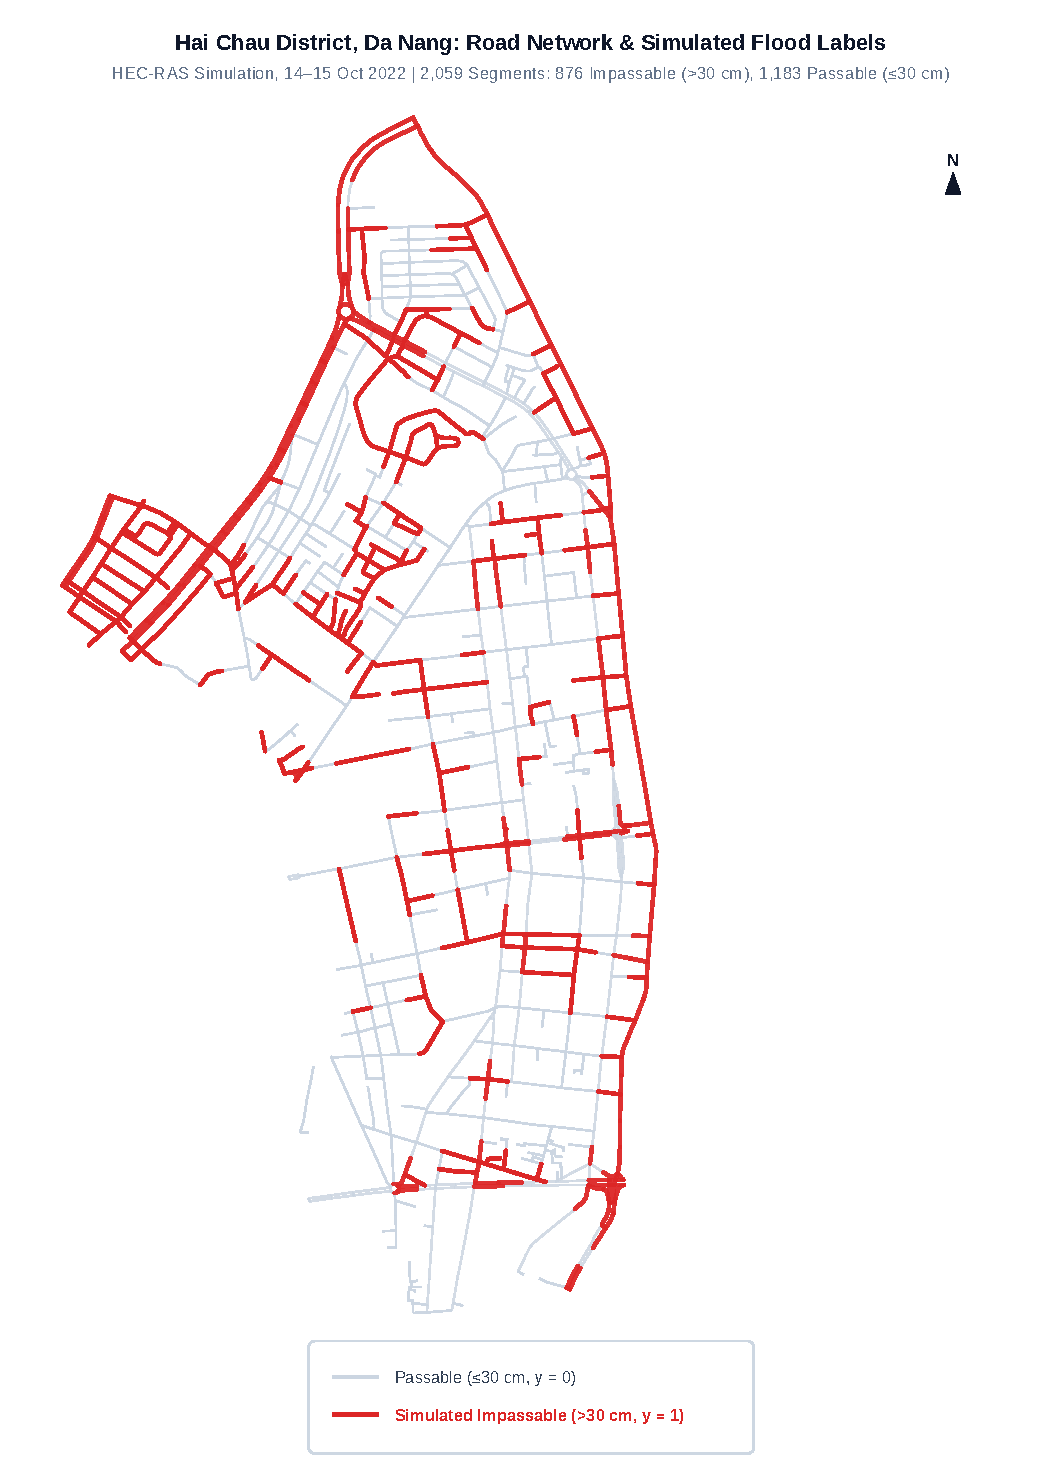
\includegraphics[width=\columnwidth]{fig1_study_area_floods}
  \caption{Study area, road network, and simulated impassable segments (water depth $>30$~cm) in Hai Chau.}
  \label{fig:studyarea}
\end{figure}

\subsection{Road Network and Flood Labels}
The drivable network was obtained from OpenStreetMap with OSMnx~\cite{boeing2017} and split at intersections and at a maximum length of 100~m, giving 1,190 intersections and 2,059 directed road segments.

Flood labels are derived from a two-dimensional HEC-RAS hydraulic simulation of 14--15 October 2022 \NRx{name the source of the HEC-RAS model and how it was calibrated or validated}. Points are sampled every 10~m along each segment centerline and matched to the nearest mesh cell, and the segment depth is the largest peak water depth over the 37 hourly time steps at these points, so a single low point can make a segment impassable. Following the 30~cm threshold of Pregnolato et al.~\cite{pregnolato2017}, segments are classed as passable ($<10$~cm; 139 segments, 6.8\%), flooded but passable (10--30~cm; 1,044 segments, 50.7\%), or impassable ($>30$~cm; 876 segments, 42.5\%).

The target is impassable flooding: $y=1$ for depth $>30$~cm and $y=0$ otherwise, so flooded-but-passable segments count as non-flooded. Section~\ref{sec:sensitivity} tests two alternatives: excluding the flooded-but-passable segments, and labeling every segment deeper than 10~cm as flooded.

\subsection{Features}
Each segment is described by 12 numerical features and its one-hot-encoded road class. Terrain features are the minimum and mean elevation, mean slope, mean topographic position index (TPI), and maximum depression depth within a 50~m buffer, computed from a 30~m digital elevation model (DEM). The hydrological feature is the distance to the Han River and its channels. Network features are road class, segment length, node degree, edge betweenness centrality, and a flag for underpasses, tunnels, and bridges. Rainfall features are the event total and peak hourly intensity at the nearest rain gauge; because one gauge covers the whole district, they are constant across segments and carry no information in this single-event benchmark.
